\scanpage{62}
b) L'application $\Sigma^{<}(2)\xrightarrow{(p_1\circ s',\unsure{p_1b'|p_1\circ b'})}\Sigma\times\Sigma$
se factorise par $\Sigma^{<}(1)\lhook\joinrel\xrightarrow{(p_1,\uline{b})}\Sigma\times\Sigma$
en un morphisme
\[
p_2:\Sigma^{<}(2)-\Sigma^{<}(1)
\]
qui rende le carré
\diagram{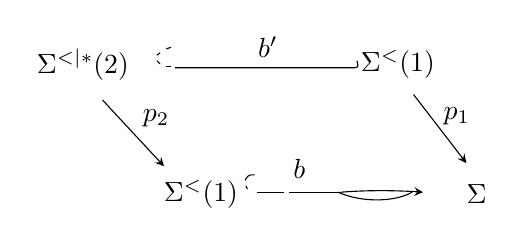
\begin{tikzpicture}[x=1cm,y=1cm,>=stealth]
\node at (0,0) {$\Sigma^{\unsure{<|*}}(2)$};
\node at (4,0) {$\Sigma^{<}(1)$};
\node at (1.5,-1.65) {$\Sigma^{<}(1)$};
\node at (5,-1.65) {$\Sigma$};
% Four separated upper hook fragments.
\draw[line width=.4pt] (1.12,.22)--(1.06,.20);
\draw[line width=.4pt] (.98,.15)--(.94,.12);
\draw[line width=.4pt] (.94,.05)--(.98,.01);
\draw[line width=.4pt] (1.05,-.02)--(1.12,-.02);
% Unheaded upper shaft, with its upturned endpoint.
\draw (1.17,-.04)--(3.45,-.04) .. controls (3.5,-.04) and (3.5,-.01) .. (3.48,.05);
\node at (2.35,.22) {$\uline{b}'$};
\draw[->] (.25,-.45)--(1.03,-1.29);
\node at (.93,-.68) {$p_2$};
\draw[->] (4.2,-.38)--(4.87,-1.25);
\node at (4.75,-.65) {$p_1$};
% Two lower hook fragments, short first shaft segment, and a gap.
\draw (2.18,-1.40) .. controls (2.10,-1.39) and (2.08,-1.43) .. (2.06,-1.47);
\draw[line width=.4pt] (2.07,-1.54)--(2.09,-1.58);
\draw (2.21,-1.62)--(2.55,-1.62);
\draw (2.62,-1.62)--(3.28,-1.62);
% The rightward portion is retraced into an elongated open loop.
\draw[->] (3.28,-1.62) .. controls (3.65,-1.59) and (4.02,-1.60) .. (4.32,-1.62);
\draw (3.24,-1.62) .. controls (3.58,-1.77) and (4.00,-1.73) .. (4.18,-1.62);
\node at (2.75,-1.32) {$\uline{b}$};
\end{tikzpicture}}
\uline{Cartésien}, et $p_1:\Sigma^{<}(1)-\Sigma$ étant transversal
à \deleted{\unsure{l'imm}}ersion-but $\uline{b}:\Sigma^{\unsure{<|*}}(1)-\Sigma$.
\margin{\uline{NB} (Si $\Sigma$ est séparé, donc $\Sigma\times\Sigma$ séparé
sur $\Sigma$, et $\Sigma^{<}(1)\overset{\uline{b}}{-}\Sigma$
propre, il en résulte
que $\Sigma^{<}(1)-\Sigma\times\Sigma$ est
propre donc un plongement
\uline{fermé}.}
\margin{cette condition de transversalité est
peut être conséquence des autres .-}

De façon équivalente, une telle structure
est donnée par un espace topologique \inserted{séparé} $\Sigma$,
muni d'une relation d'ordre $x\preceq y$
\deleted{dont le graphe est}\inserted{satisfaisant les conditions suivantes}

% Two unassigned dark points beside the first cancelled a) line.
\margin{\figure{\begin{tikzpicture}[x=1mm,y=1mm]
\fill (0,0) circle (.16mm);
\fill (.5,-.8) circle (.16mm);
\end{tikzpicture}}}
\deleted{a) le graphe \deleted{$\unsure{\Sigma^{<}(1)|\Sigma^{*}(1)}$} $\Sigma(1)$ de cette relation est
fermé dans $\Sigma\times\Sigma$, et $\Sigma(1)\overset{\uline{b}}{-}\Sigma$ est
une immersion\unsure{.}
\deleted{$\unsure{\Sigma}$}
b) Si $\Sigma^{*}(1)$ est le graphe de la
relation d'ordre \inserted{stricte}, $\Sigma^{*}(1)\xrightarrow{\uline{b}}\Sigma$ est une
immersion \inserted{bordante} propre \deleted{\unsure{(donc la partie de}}
a) Si $x\in\Sigma$, $\Sigma_{<x}$ \inserted{$(=\Sigma^{\unsure{<|*}}(1)_{\unsure{x}})$}\unsure{,}
\unsure{\deleted{\unsure{est} \unsure{un|une}}|\unsure{est} \unsure{un|une}}
\unsure{ens|est} (fini) \uline{tot}$ {}^t$. \uline{ordonné}.
}
\margin{\handwritten{61}}
